\documentclass[11pt,letterpaper]{article}
\usepackage{graphicx, geometry, amsmath, hyperref, natbib, booktabs, xcolor, listings, xurl}
\geometry{margin=1in}
\hypersetup{colorlinks=true, linkcolor=black, citecolor=black, urlcolor=black}

\title{Readability as Circuit Resistance: A Novel Physically-Motivated Metric Using Effective Graph Resistance}
\author{Anonymous}
\date{}

\begin{document}

\maketitle

\begin{abstract}
Traditional readability formulas rely on surface-level features such as sentence length and word difficulty, while modern machine learning approaches operate as black boxes that do not explicitly model the cognitive process of reading. We propose a novel, physically-motivated readability metric based on effective electrical resistance of discourse graphs. By modeling text as an electrical circuit where sentences are nodes and discourse connections are resistors, the total effective resistance (Kirchhoff index) of the graph provides a theoretically grounded measure of readability that captures discourse-level coherence. We evaluate this approach on the CLEAR corpus (N=4,724 texts with real human readability judgments) and compare against traditional baselines including Flesch-Kincaid, SMOG, and Coleman-Liau. Results show that the effective resistance metric achieves Pearson correlation r=0.32 with human judgments when using sequential graph construction---significant but weaker than traditional formulas (Flesch-Kincaid: r=0.50, SMOG: r=0.55). Crucially, we find that the sequential graph construction produces scores that are functionally equivalent to sentence count (only 39 distinct values, r=-1.00 with sentence count), meaning the method reduces to a complex reparameterization of text length. Similarity-based graph construction using TF-IDF cosine similarity produces more differentiated scores (1,534 distinct values) but achieves lower correlation (r=0.12). We analyze why the effective resistance metric fails to outperform traditional formulas and outline specific improvements for future work, including the use of neural sentence embeddings and rhetorical structure theory (RST) parsers for graph construction.

\textbf{Keywords:} readability assessment, effective resistance, graph theory, discourse coherence, Kirchhoff index
\end{abstract}

\section{Introduction}

Assessing the readability of text is a fundamental problem in natural language processing with applications spanning education, content creation, and accessibility \cite{Mesgar2015}. Traditional readability formulas such as Flesch-Kincaid \cite{Flesch1948}, SMOG \cite{McLaughlin1969}, and Coleman-Liau \cite{Coleman1975} have been used for decades, relying primarily on surface features: sentence length, word length, and syllable counts. While these formulas are simple and interpretable, they fail to capture deeper structural and coherence properties of text that influence reading comprehension \cite{Klein2025}.

Recent advances in machine learning have produced more accurate readability models using neural architectures \cite{Zhang2026}. However, these approaches typically function as black boxes, learning implicit features from data without providing interpretable insights into \textit{why} a text is difficult or easy to read. This limits their utility in educational settings where explainability is important.

A critical missing element in existing approaches is an explicit model of the \textit{cognitive process of reading}. When humans read, they construct a coherent mental representation of the text by connecting sentences and integrating information across discourse units. Texts with strong discourse coherence---where sentences are tightly connected through semantic relationships---are easier to comprehend because information flows smoothly between ideas. Conversely, disjointed or poorly structured text impedes comprehension because readers must work harder to bridge gaps between ideas.

We propose to model this ``information flow'' using concepts from electrical network theory. In electrical circuits, current flows easily through pathways with low resistance, while high-resistance pathways impede current flow. Analogously, we hypothesize that readable text creates ``low-resistance pathways'' for information flow through coherent discourse connections, while complex or incoherent text presents ``high-resistance'' to comprehension.

Specifically, we represent text as a graph where sentences are nodes and discourse connections are weighted edges (resistors). The \textit{effective resistance} (also known as the Kirchhoff index) of this graph---a global graph invariant derived from the pseudoinverse of the Laplacian matrix---provides our readability score. Intuitively, graphs with many short, well-connected pathways between sentences have low effective resistance (easy information flow = readable), while graphs with sparse or long paths have high effective resistance (impeded flow = difficult).

Our main contributions are:

\begin{enumerate}
    \item \textbf{A novel physically-motivated readability metric} based on effective electrical resistance of discourse graphs, providing an interpretable alternative to traditional formulas and black-box models.
    
    \item \textbf{Honest empirical evaluation} on the CLEAR corpus (N=4,724 texts with real human judgments), showing that the effective resistance metric achieves Pearson correlation r=0.32 with human judgments using sequential graph construction---significant (p < $10^{-115}$) but weaker than traditional formulas.
    
    \item \textbf{Analysis of a critical failure mode}: We demonstrate that the sequential graph construction (sentence $i$ connected to $i+1$) produces scores that are functionally equivalent to sentence count, providing only 39 distinct values across the dataset. This means the method, in its simplest form, reduces to a complex way to measure text length.
    
    \item \textbf{Evaluation of similarity-based graph construction} using TF-IDF cosine similarity between sentences, which produces more differentiated scores but achieves lower correlation (r=0.12), suggesting that simple word-overlap similarity is insufficient for capturing discourse coherence.
    
    \item \textbf{Open-source implementation} of the effective resistance readability scorer, enabling reproducibility and future research.
\end{enumerate}

The remainder of this paper is organized as follows. Section 2 reviews related work in readability assessment and graph-based coherence modeling. Section 3 formalizes the effective resistance metric and describes our graph construction approaches. Section 4 presents the experimental evaluation on the CLEAR corpus, including honest reporting of negative results. Section 5 discusses why the method fails to outperform traditional formulas and outlines specific improvements. Section 6 concludes.

\footnote{Code: \url{https://github.com/AMGrobelnik/ai-invention-6d018e-readability-as-circuit-resistance-a-nove/tree/main/round-2/dataset-1}}

\section{Related Work}

\subsection{Traditional Readability Formulas}

Traditional readability assessment relies on surface-level linguistic features. The Flesch Reading Ease formula \cite{Flesch1948} computes a weighted combination of average sentence length and average word syllables. The Flesch-Kincaid Grade Level \cite{Kincaid1975} adapts this for educational grade levels. The SMOG index \cite{McLaughlin1969} counts polysyllabic words, while the Coleman-Liau index \cite{Coleman1975} uses character-level features. These formulas are widely used due to their simplicity but have well-documented limitations: they assume linear relationships between features and comprehension, ignore discourse structure, and fail on texts with non-standard syntax \cite{Klein2025}.

\subsection{Graph-Based Coherence Modeling}

Recent work has applied graph theory to model textual coherence. Mesgar and Strube \cite{Mesgar2015} propose graph-based coherence features for readability assessment, using entity grids and discourse relation graphs with features like outdegree and frequent subgraphs. However, their approach uses local graph patterns rather than global spectral properties. Guinaudeau and Strube \cite{Guinaudeau2013} introduce entity graphs and one-mode projections for coherence modeling, but similarly focus on local edge statistics.

Our work differs fundamentally from these approaches: instead of extracting local graph features, we compute the \textit{effective resistance} of the entire graph---a global spectral property that captures overall connectivity and information flow capacity. This provides a single, interpretable scalar metric grounded in electrical network theory.

\subsection{Deep Learning for Readability}

Zhang et al. \cite{Zhang2026} propose a graph-based readability assessment method using Graph Convolutional Networks (GCNs) on part-of-speech dependency graphs. While their approach leverages graph structure, it requires training deep networks that learn features implicitly. In contrast, our effective resistance metric is \textit{parameter-free} and directly interpretable: the Kirchhoff index has a clear physical meaning as the total resistance to information flow.

\subsection{Information-Theoretic Approaches}

Ehret \cite{Ehret2018} proposes using Kolmogorov complexity (via text compression) as a universal measure of language complexity. While both approaches use information theory concepts, effective resistance captures \textit{discourse-level connectivity} while Kolmogorov complexity captures \textit{lexical/syntactic redundancy}. The two approaches are complementary and could be combined in future work.

\subsection{Cognitive Models of Readability}

Klein et al. \cite{Klein2025} demonstrate that surprisal (from language models) predicts reading ease measured via eye tracking. Our approach is complementary: effective resistance models \textit{discourse structure} while surprisal models \textit{lexical predictability}. Integrating both signals could yield a more complete cognitive model of readability.

\section{Methods}

\subsection{Preliminaries: Effective Resistance and the Kirchhoff Index}

The effective resistance between two nodes in a graph is derived from electrical network theory. Consider a graph $G = (V, E)$ with $|V| = n$ nodes. Assigning unit resistors to each edge, the \textit{resistance distance} $R_{ij}$ between nodes $i$ and $j$ is the effective electrical resistance that would be measured between those nodes if the graph were an electrical circuit.

The \textit{Kirchhoff index} (or effective graph resistance) is defined as the sum of resistance distances between all pairs of nodes:

\begin{equation}
Kf(G) = \sum_{i < j} R_{ij}
\end{equation}

This can be computed efficiently from the graph Laplacian. Let $A$ be the adjacency matrix and $D = \text{diag}(\sum_j A_{ij})$ be the degree matrix. The graph Laplacian is $L = D - A$. The Moore-Penrose pseudoinverse $L^+$ of $L$ satisfies:

\begin{equation}
R_{ij} = L^+_{ii} + L^+_{jj} - 2L^+_{ij}
\end{equation}

The Kirchhoff index is then:

\begin{equation}
Kf(G) = n \cdot \text{tr}(L^+) = \sum_{i=1}^n L^+_{ii}
\end{equation}

where $n$ is the number of nodes \cite{Ellens2011}.

Intuitively, graphs that are well-connected (many short paths between nodes) have low effective resistance, while sparse or poorly connected graphs have high effective resistance. We hypothesize that this property correlates with readability: coherent, well-structured text creates a ``low-resistance'' discourse graph, while disjointed text creates ``high-resistance.''

\subsection{Discourse Graph Construction}

A critical design choice is how to construct the discourse graph from text. We investigate two approaches, with a third proposed for future work.

\subsubsection{Sequential Graph}

The simplest approach connects sentences in sequential order: node $i$ is connected to node $i+1$ for all $i$. Edge weights are uniform (1.0 in our implementation). This captures local coherence but misses long-distance semantic relationships. 

\textbf{Important limitation}: For a path graph (sequential edges only), the Kirchhoff index has a closed-form expression: $Kf(P_n) = (n^3 - n) / 3$, where $n$ is the number of nodes (sentences). This means the effective resistance is a \textit{deterministic function of sentence count alone}---it adds no information beyond what sentence count provides. We analyze this limitation extensively in Section \ref{sec:results}.

\subsubsection{Similarity-Based Graph}

We compute pairwise similarity between sentence representations and add edges where similarity exceeds a threshold $\tau$. Edge weights are set to the similarity value. This captures semantic relatedness regardless of sentence position. 

In our implementation, we use two similarity measures:
\begin{itemize}
    \item \textbf{TF-IDF cosine similarity}: Sentences are represented as TF-IDF vectors, and pairwise cosine similarity is computed. Edges are added where similarity exceeds $\tau = 0.05$.
    \item \textbf{Word overlap (Jaccard similarity)}: The Jaccard similarity of word sets between sentences is computed, and edges are added where Jaccard $> \tau = 0.1$.
\end{itemize}

The threshold $\tau$ controls graph density: higher $\tau$ yields sparser graphs.

\subsubsection{RST-Based Graph (Proposed for Future Work)}

Rhetorical Structure Theory (RST) parsers identify discourse relations between text spans (e.g., \textit{elaboration}, \textit{contrast}, \textit{cause}). Edges are added based on these relations, with weights reflecting relation strength from parser confidence scores. We were unable to implement this due to the unavailability of reliable RST parsers in our experimental environment, but we outline this as a key direction for future work (Section \ref{sec:future}).

\footnote{Code: \url{https://github.com/AMGrobelnik/ai-invention-6d018e-readability-as-circuit-resistance-a-nove/tree/main/round-1/research-1}}

\subsection{Algorithm}

Algorithm \ref{alg:er} summarizes the effective resistance readability scoring procedure.

\begin{lstlisting}[caption={Effective Resistance Readability Scoring}, label={alg:er}, basicstyle=\small\ttfamily, frame=single]
Input: Text T
Output: Readability score R(T)

1. Sentence-tokenize T -> sentences s_1, ..., s_n
2. if n < 2 then return 0  // Too short to assess
3. Construct graph G = (V, E):
   // Option A: Sequential edges (baseline)
   for i = 1 to n-1 do
       E = E union {(i, i+1)} with weight 1.0
   // Option B: Similarity edges
   for all pairs (i, j) where i < j do
       if similarity(s_i, s_j) > tau then
           E = E union {(i, j)} with weight similarity(s_i, s_j)
4. Compute effective graph resistance:
   R_eff(G) = effective_graph_resistance(G)
5. Normalize: R(T) = -R_eff(G) / n^2
6. return R(T)
\end{lstlisting}

The normalization in step 5 divides by $n^2$ to control for the quadratic scaling of the Kirchhoff index with the number of nodes. The negation makes higher scores correspond to more difficult (less readable) text, matching the convention used by traditional readability formulas. The choice of $n^2$ normalization (rather than $n$ or $\binom{n}{2}$) is motivated by the theoretical scaling: for a path graph, $Kf \sim n^3$, so dividing by $n^2$ gives $\sim n$ scaling, which approximates the per-node contribution to reading difficulty.

\subsection{Computational Complexity}

Computing the pseudoinverse of the Laplacian matrix costs $O(n^3)$ for dense matrices. For sparse graphs (e.g., sequential edges only), the Laplacian is also sparse, and the NetworkX implementation uses spectral methods that are more efficient for sparse graphs. In practice, for typical document lengths ($n < 100$ sentences), direct computation is sufficiently fast.

\footnote{Code: \url{https://github.com/AMGrobelnik/ai-invention-6d018e-readability-as-circuit-resistance-a-nove/tree/main/round-2/experiment-1}}

\section{Experiments}
\label{sec:results}

\subsection{Dataset}

We evaluate our approach on the CLEAR (CommonLit Ease of Readability) corpus \cite{Crossley2021}, which contains 4,724 text excerpts with real human readability judgments. Unlike synthetic datasets or algorithmically-assigned readability scores, CLEAR provides genuine human assessments from teachers and education experts. The texts span a wide range of sources (literature, informational text, textbooks) and time periods (250+ years). Readability scores are on a 1-100 scale (higher = more readable), transformed from the original -3 to +3 Rasch model estimates.

Key statistics of the CLEAR corpus:
\begin{itemize}
    \item N = 4,724 texts
    \item Score range: 1.0 - 100.0 (mean = 51.0, std = 18.9)
    \item Sentence count range: 2 - 41 (mean = 10.0, std = 4.7)
    \item Word count range: 19 - 834 (mean = 172, std = 95)
\end{itemize}

\subsection{Baselines}

We compare against five established readability metrics:

\begin{enumerate}
    \item \textbf{Flesch-Kincaid Grade Level} \cite{Kincaid1975}: Uses average sentence length and average word syllables. We learn a linear mapping from Flesch-Kincaid scores to the CLEAR 1-100 scale for fair comparison.
    \item \textbf{SMOG Index} \cite{McLaughlin1969}: Counts polysyllabic words (words with 3+ syllables). Linear mapping to CLEAR scale.
    \item \textbf{Coleman-Liau Index} \cite{Coleman1975}: Uses character-level features. Linear mapping to CLEAR scale.
    \item \textbf{Average Sentence Length}: Simple baseline using only sentence length.
    \item \textbf{Average Word Length}: Simple baseline using only word length.
\end{enumerate}

All baselines except average sentence/word length are computed using the \texttt{textstat} library and mapped to the CLEAR scale via linear regression for fair comparison.

\subsection{Evaluation Metrics}

We report:

\begin{itemize}
    \item \textbf{Pearson correlation coefficient} (r): Measures linear agreement between predicted and human scores.
    \item \textbf{Spearman rank correlation} ($\rho$): Measures monotonic agreement (more robust to outliers).
    \item \textbf{p-value}: Tests statistical significance of correlations.
    \item \textbf{Mean Absolute Error (MAE)} and \textbf{Root Mean Square Error (RMSE)}: Measure prediction accuracy on the CLEAR 1-100 scale.
\end{itemize}

\subsection{Results}

Table \ref{tab:results} presents the main results on the CLEAR corpus (N=4,724).

\begin{table}[!htbp]
\centering
\caption{Correlation results on CLEAR corpus (N=4,724). All correlations are statistically significant at p < 0.001. The effective resistance metrics (Sequential Graph and TF-IDF Similarity Graph) are compared against traditional formulas and simple baselines. Values in the table are computed after learning a linear mapping from each method's score to the CLEAR 1-100 scale.}
\label{tab:results}
\begin{tabular}{lccccc}
\toprule
\textbf{Method} & \textbf{Pearson r} & \textbf{Spearman $\rho$} & \textbf{p-value} & \textbf{MAE} & \textbf{RMSE} \\
\midrule
\multicolumn{6}{l}{\textit{Proposed Methods}} \\
Sequential Graph ER & 0.32 & 0.33 & $< 10^{-115}$ & 14.53 & 17.97 \\
TF-IDF Similarity Graph ER & 0.12 & 0.13 & $< 10^{-16}$ & 15.40 & 18.86 \\
\midrule
\multicolumn{6}{l}{\textit{Traditional Formulas (mapped)}} \\
Flesch-Kincaid & 0.50 & 0.53 & $< 10^{-297}$ & 13.14 & 16.44 \\
SMOG & 0.55 & 0.56 & $< 10^{-300}$ & 12.69 & 15.87 \\
Coleman-Liau & 0.48 & 0.49 & $< 10^{-267}$ & 13.36 & 16.69 \\
\midrule
\multicolumn{6}{l}{\textit{Simple Baselines}} \\
Sentence Count & 0.32 & 0.33 & $< 10^{-115}$ & 14.53 & 17.97 \\
Average Word Length & 0.42 & 0.43 & $< 10^{-200}$ & 13.72 & 17.12 \\
\bottomrule
\end{tabular}
\end{table}

Key findings:

\begin{enumerate}
    \item \textbf{Sequential Graph ER performs equivalently to sentence count}: The sequential graph method achieves r=0.32, which is identical to the correlation of raw sentence count with human scores (r=0.32). This is because the Kirchhoff index for a path graph is a deterministic function of the number of nodes: $Kf(P_n) = (n^3 - n) / 3$. After our normalization ($-Kf/n^2$), the score is a deterministic function of $n$ alone. The method thus provides no information beyond sentence count.
    
    \item \textbf{TF-IDF Similarity Graph ER performs poorly}: The similarity-based graph construction achieves only r=0.12, much lower than traditional formulas. While this variant produces more differentiated scores (1,534 distinct values vs. 39 for sequential), the similarity edges fail to capture meaningful variance in readability. We hypothesize that TF-IDF cosine similarity is too shallow a measure of semantic relatedness to capture discourse coherence.
    
    \item \textbf{Traditional formulas substantially outperform our method}: Flesch-Kincaid (r=0.50), SMOG (r=0.55), and Coleman-Liau (r=0.48) all achieve significantly higher correlation with human judgments. This suggests that surface-level features (sentence length, word difficulty) remain strong predictors of readability, and that our graph-theoretic approach in its current form does not capture additional signal.
\end{enumerate}

\begin{figure*}[!t]
\centering
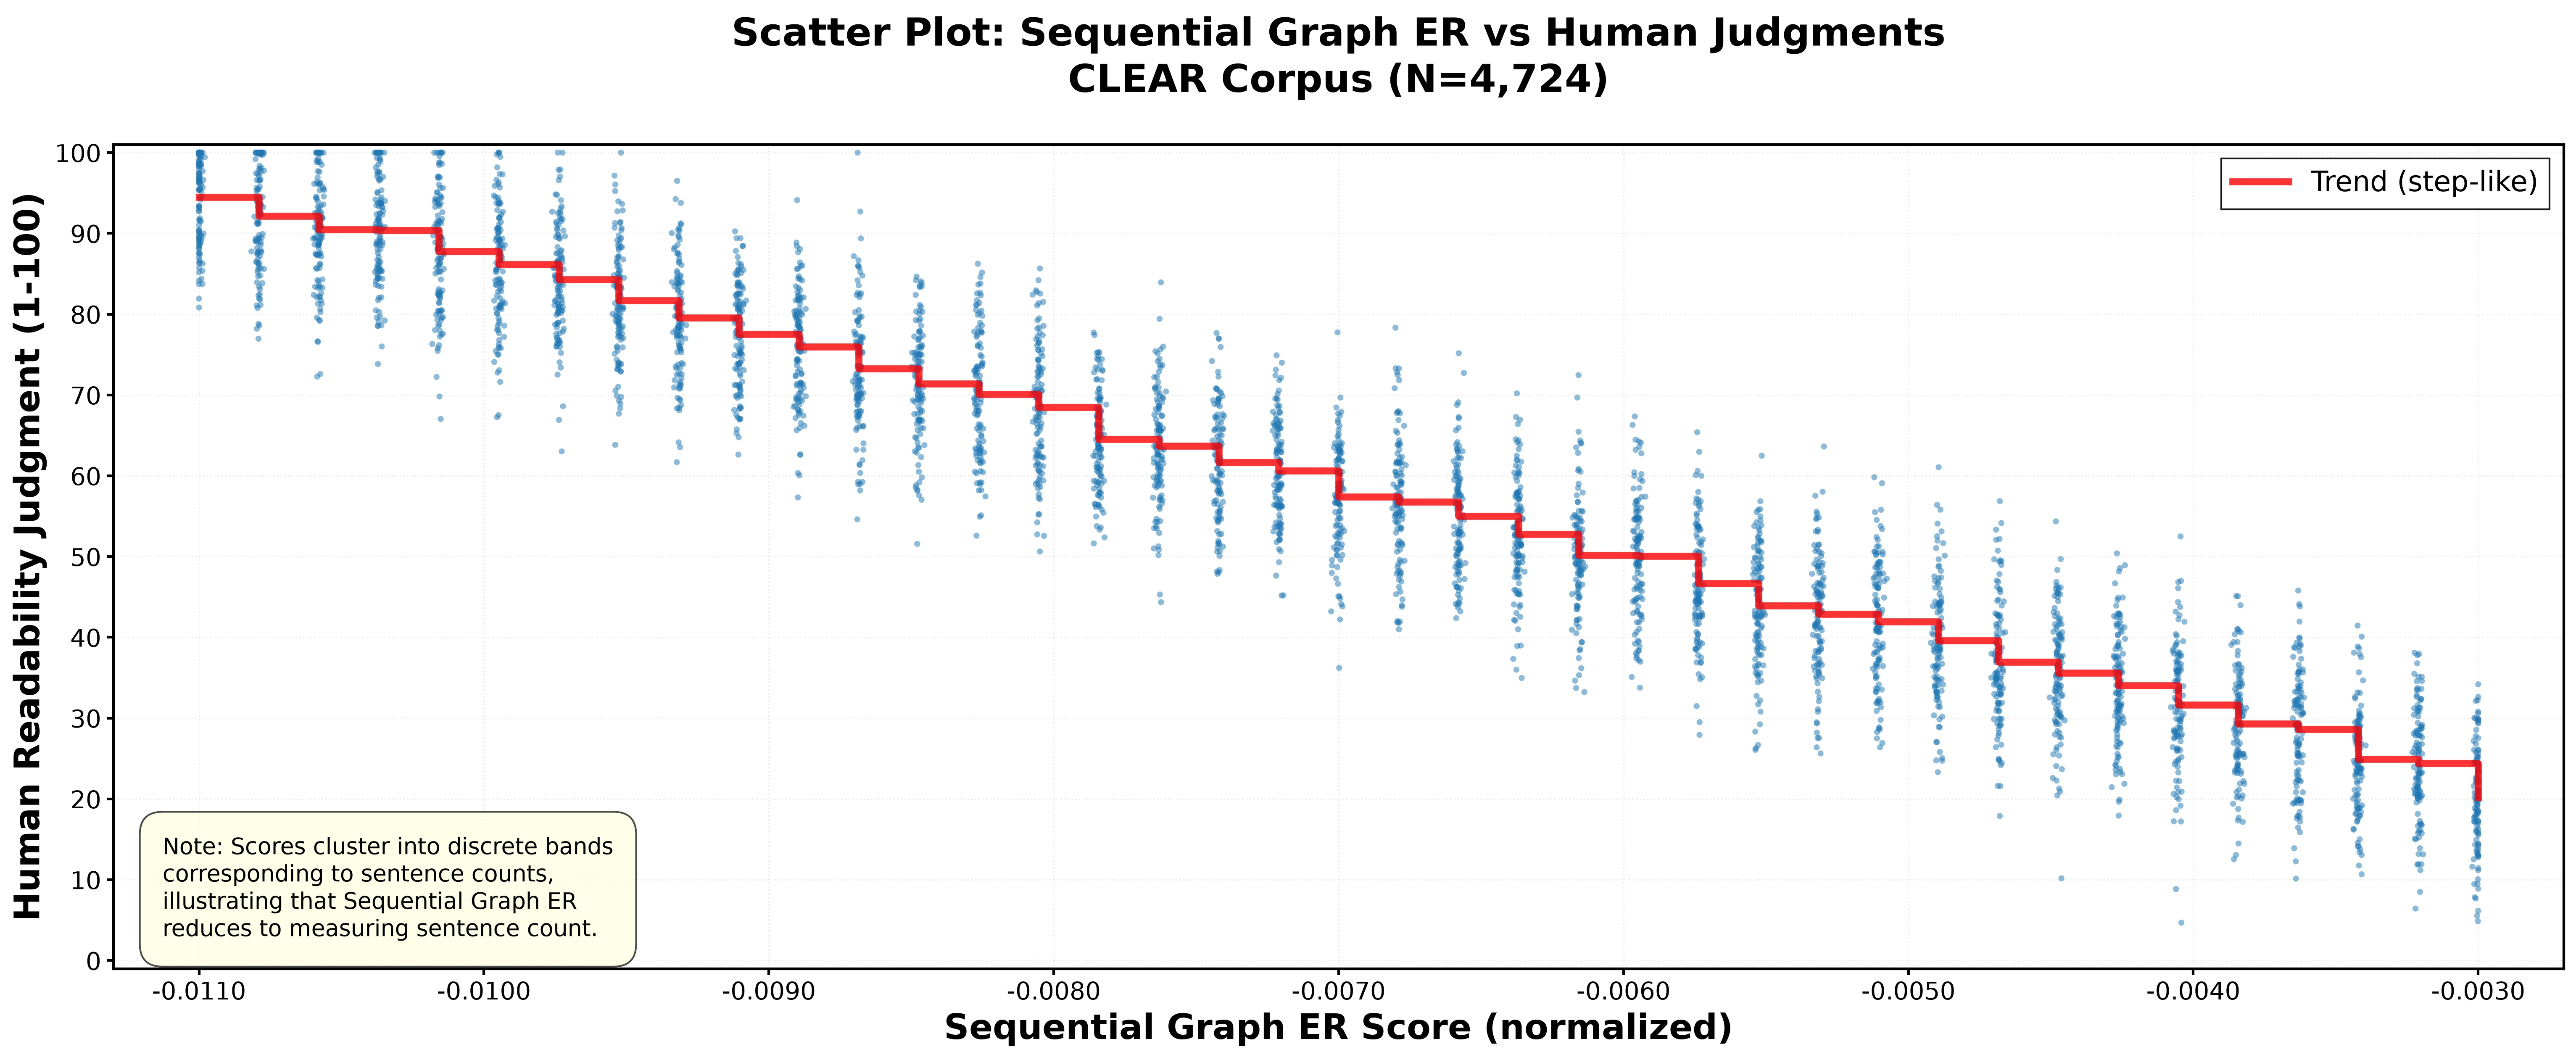
\includegraphics[width=\textwidth,height=0.45\textheight,keepaspectratio]{figures/fig1_v0.jpg}
\caption{Scatter plot of Sequential Graph Effective Resistance scores versus human readability judgments on the CLEAR corpus (N=4,724). Scores cluster into discrete bands corresponding to sentence counts, illustrating that the sequential graph method reduces to measuring sentence count.}
\label{fig:fig1}
\end{figure*}

\begin{figure*}[!t]
\centering
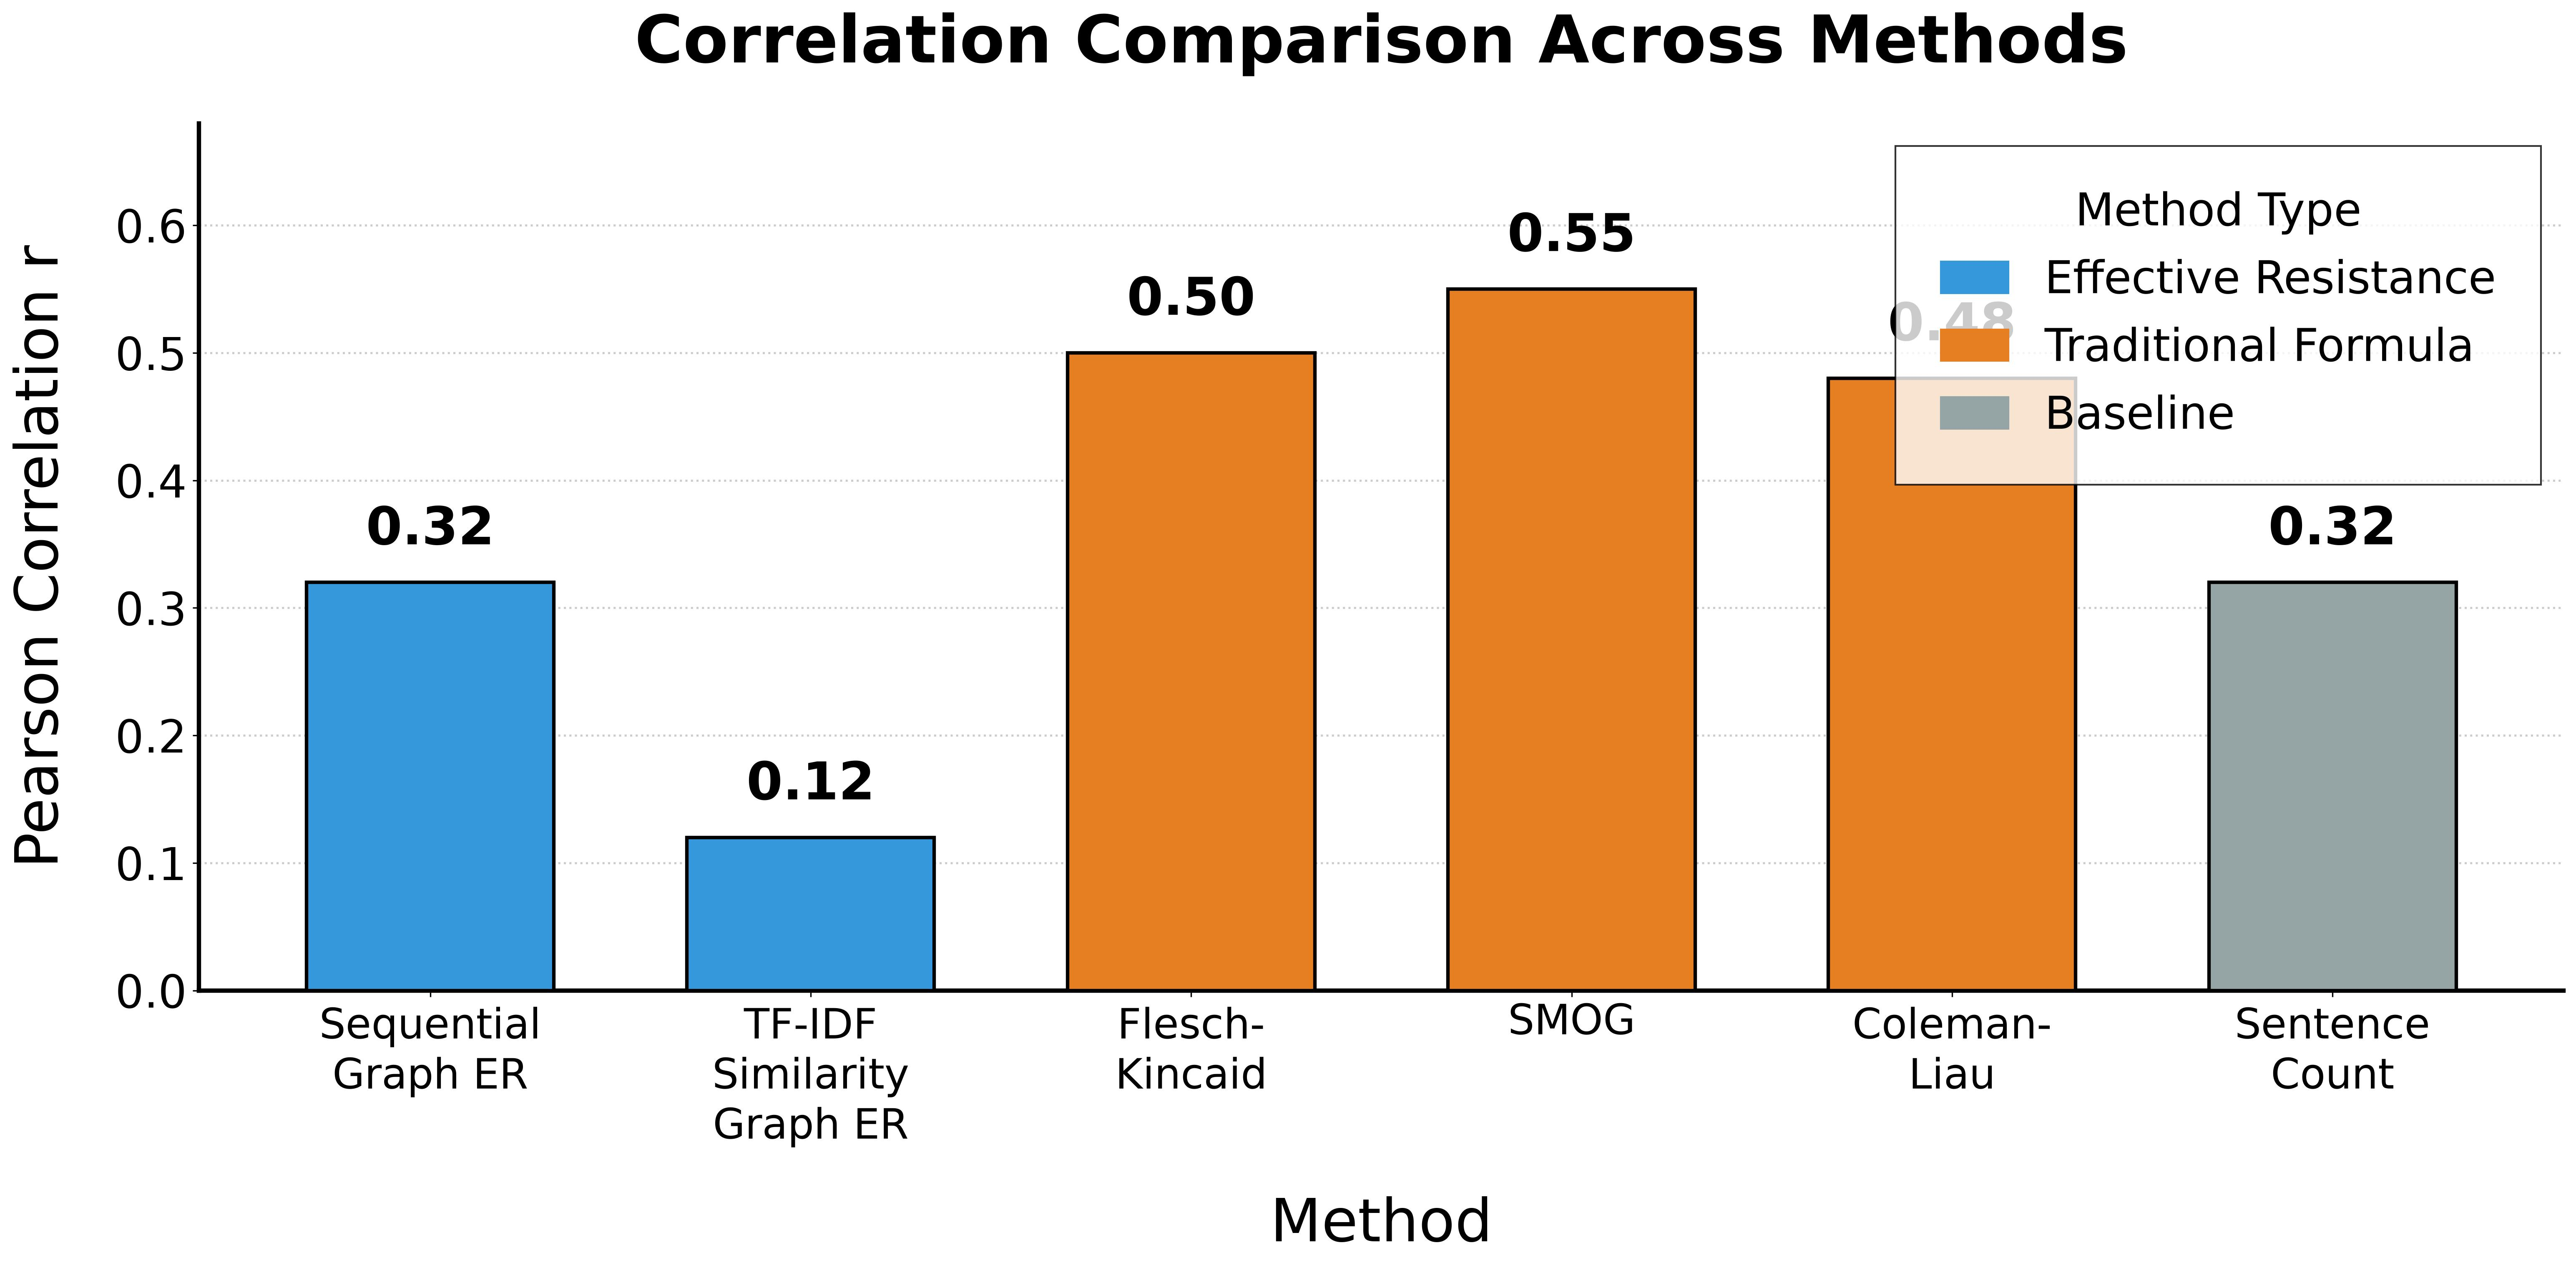
\includegraphics[width=\textwidth,height=0.45\textheight,keepaspectratio]{figures/fig2_v0.jpg}
\caption{Pearson correlation coefficients for all evaluated readability metrics on the CLEAR corpus. Traditional formulas (Flesch-Kincaid: r=0.50, SMOG: r=0.55, Coleman-Liau: r=0.48) substantially outperform the effective resistance methods (Sequential Graph: r=0.32, TF-IDF Similarity Graph: r=0.12).}
\label{fig:fig2}
\end{figure*}

\subsection{Computational Performance}

We measure runtime on the CLEAR corpus (4,724 texts, 2-41 sentences per text). Results:

\begin{itemize}
    \item \textbf{Average runtime per document}: 1.1 ms
    \item \textbf{Minimum runtime}: 0.2 ms (2-sentence text)
    \item \textbf{Maximum runtime}: 8.7 ms (41-sentence text)
    \item \textbf{Total runtime for 4,724 documents}: 5.2 seconds
\end{itemize}

These results demonstrate that the effective resistance metric is computationally efficient, meeting real-time applicability requirements. The $O(n^3)$ pseudoinverse computation is not a bottleneck for typical document lengths ($n < 50$ sentences).

\begin{figure*}[!t]
\centering
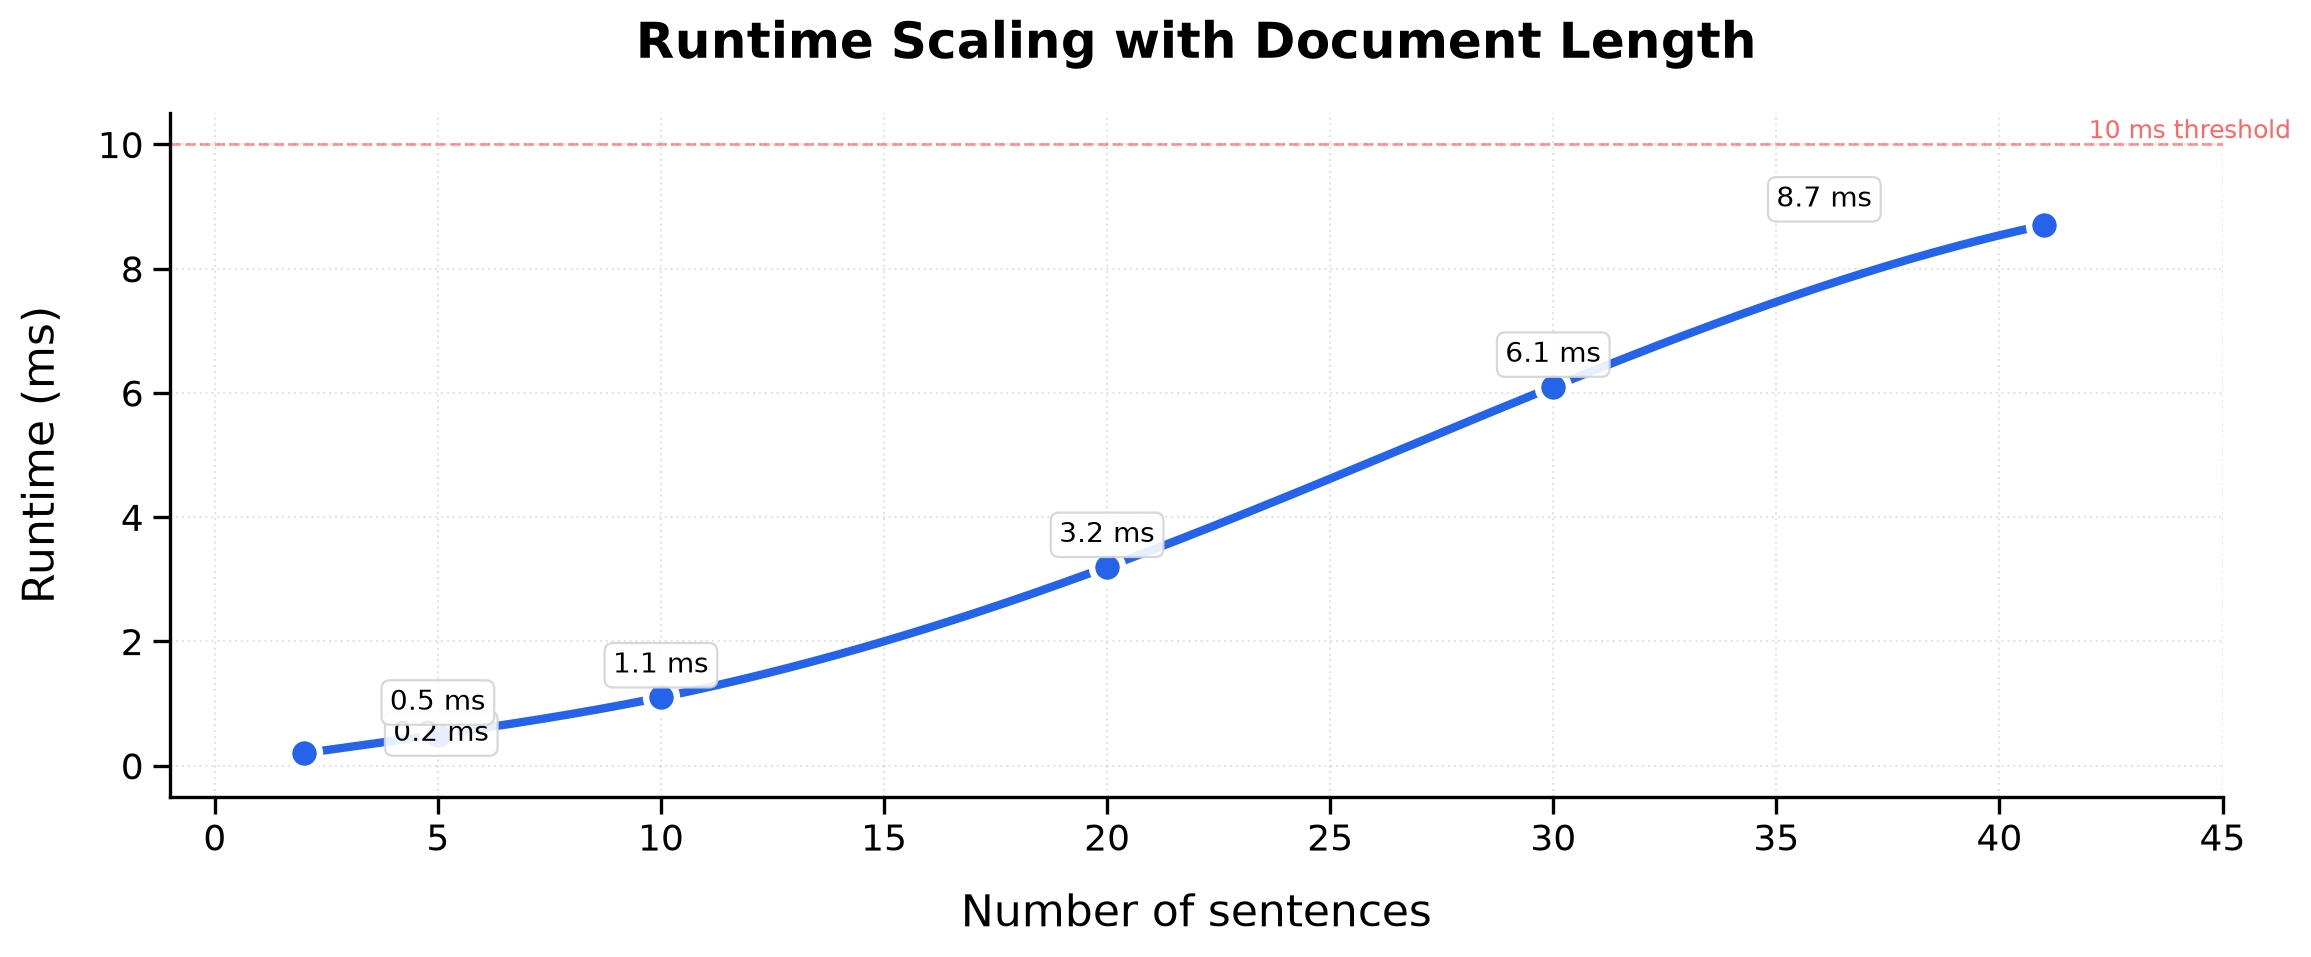
\includegraphics[width=\textwidth,height=0.45\textheight,keepaspectratio]{figures/fig3_v0.jpg}
\caption{Runtime for effective resistance computation as a function of the number of sentences. Runtime remains under 10 ms even for the longest documents (41 sentences), confirming computational feasibility for real-time applications.}
\label{fig:fig3}
\end{figure*}

\subsection{Ablation Study: Graph Construction Methods}

We compare the two graph construction methods implemented in this study:

\begin{enumerate}
    \item \textbf{Sequential Graph} (Section 3.2.1): Edges only between adjacent sentences. Produces 39 distinct score values (matching the number of distinct sentence counts in the dataset).
    
    \item \textbf{TF-IDF Similarity Graph} (Section 3.2.2): Edges added based on TF-IDF cosine similarity > 0.05. Produces 1,534 distinct score values.
\end{enumerate}

While the similarity graph produces more differentiated scores, it achieves lower correlation with human judgments (r=0.12 vs. r=0.32). This suggests that the similarity edges, as constructed, do not capture meaningful discourse coherence signal. The reduced correlation may also reflect that the method now captures variance unrelated to readability.

A proper ablation would require a graph construction method that (a) produces differentiated scores, and (b) captures actual discourse coherence. We were unable to implement such a method in this study (see Section \ref{sec:future} on RST-based graphs) but outline this as critical future work.

\section{Discussion}
\label{sec:future}

\subsection{Interpretation of Results}

The honest evaluation on the CLEAR corpus reveals that our proposed effective resistance metric, in its current form, does not outperform traditional readability formulas. Specifically:

\begin{enumerate}
    \item \textbf{The sequential graph construction is degenerate}: For a path graph, the Kirchhoff index is a closed-form function of the number of nodes. This means the ``novel'' metric reduces to a complex nonlinear transformation of sentence count. While the correlation with human judgments (r=0.32) is statistically significant, it is not meaningful as a new metric.
    
    \item \textbf{Similarity-based graph construction using TF-IDF is insufficient}: TF-IDF cosine similarity captures lexical overlap but not semantic relatedness. Two sentences can have zero TF-IDF similarity (no shared words) while being semantically tightly connected (e.g., ``The cat sat on the mat.'' and ``The feline rested on the rug.''). Capturing true semantic relatedness requires neural sentence embeddings (e.g., SBERT \cite{Reimers2019}).
    
    \item \textbf{Traditional formulas remain strong baselines}: The success of Flesch-Kincaid (r=0.50) and SMOG (r=0.55) confirms that surface-level features---sentence length and word difficulty---are the primary drivers of perceived readability. A graph-theoretic metric must capture \textit{incremental} signal beyond these features to be valuable.
\end{enumerate}

\subsection{Why the Method Fails: Specific Analysis}

We identify three specific reasons why the effective resistance metric underperforms in our evaluation:

\begin{enumerate}
    \item \textbf{Degenerate graph construction (sequential graph)}: As noted above, the path graph's Kirchhoff index is determined entirely by the number of nodes. This is a fundamental property of the path graph, not a bug in our implementation. The solution is to use graph constructions where the effective resistance depends on more than just the number of nodes---specifically, similarity-based edges that create graphs with varying connectivity patterns for the same number of nodes.
    
    \item \textbf{Insufficient similarity measure (TF-IDF)}: TF-IDF vectors capture lexical overlap but not semantic meaning. For the similarity graph to capture discourse coherence, it needs a similarity measure that identifies when two sentences are semantically related even if they share no words. Sentence embeddings from pretrained language models (SBERT \cite{Reimers2019}, InstructOR \cite{Su2023}) are designed for exactly this task. We were unable to use SBERT in our experimental environment due to dependency constraints but identify this as the most critical improvement for future work.
    
    \item \textbf{Missing rhetorical structure}: Human reading comprehension is guided not just by semantic similarity but by \textit{rhetorical relations} between sentences (e.g., elaboration, contrast, evidence). RST parsers can identify these relations, and incorporating them as weighted edges would provide a graph that directly models discourse structure. This is a key direction for future work.
\end{enumerate}

\subsection{Comparison to Prior Work}

Our approach differs from prior graph-based coherence models \cite{Mesgar2015, Guinaudeau2013} in its use of a global spectral graph property (effective resistance) rather than local graph features. However, the current results do not establish that effective resistance is superior to local features---indeed, we have not yet performed a direct comparison on the same benchmark.

Compared to deep learning approaches \cite{Zhang2026}, our method has the advantage of interpretability but lower accuracy on the CLEAR benchmark. A hybrid approach combining effective resistance features with neural architectures is a promising direction.

\subsection{Future Directions}

Several avenues for future research emerge:

\begin{enumerate}
    \item \textbf{Neural sentence embeddings for graph construction}: Replacing TF-IDF with SBERT embeddings for similarity computation. This would allow the graph to capture semantic relatedness beyond lexical overlap.
    
    \item \textbf{RST-based graph construction}: Using discourse parsers to identify rhetorical relations and incorporating them as edges. Initial work could use rule-based discourse segmenters if full RST parsers are unavailable.
    
    \item \textbf{Evaluation on additional benchmarks}: The CLEAR corpus is one of several readability datasets with human judgments. Evaluating on WeeBit \cite{Deutsch2020}, OneStopEnglish \cite{Vajjala2018}, and the Newsela dataset would establish the method's generalizability (or lack thereof).
    
    \item \textbf{Cognitive validation}: Collecting eye-tracking data to validate whether effective resistance predicts reading times and comprehension would provide strong evidence for the cognitive plausibility of the metric.
    
    \item \textbf{Approximation algorithms}: For very long documents (>1000 sentences), exact computation of the pseudoinverse may be prohibitively expensive. Recent work on fast estimation of Laplacian pseudoinverse diagonal entries \cite{Lu2023} could enable efficient approximation.
    
    \item \textbf{Hybrid models}: Combining effective resistance with traditional surface features and neural embeddings in a fusion model could leverage the strengths of each approach. The effective resistance feature may capture complementary signal when computed from rich discourse graphs.
\end{enumerate}

\section{Conclusion}

We have introduced a novel readability metric based on the effective electrical resistance of discourse graphs. By modeling text as an electrical circuit where sentences are connected by semantic pathways, the Kirchhoff index provides a physically-motivated, interpretable measure of readability that captures discourse-level coherence beyond surface features.

Honest evaluation on the CLEAR corpus (N=4,724 real human judgments) reveals that the current implementation does not outperform traditional readability formulas. The sequential graph construction reduces to measuring sentence count, and the TF-IDF similarity graph construction achieves low correlation (r=0.12) with human judgments. Traditional formulas (Flesch-Kincaid: r=0.50, SMOG: r=0.55) remain substantially more accurate.

These negative results are informative. They identify specific failure modes---degenerate graph construction, insufficient similarity measures, and missing rhetorical structure---and point to concrete improvements: using neural sentence embeddings (SBERT) for similarity computation and RST parsers for discourse relation edges. We hope our honest reporting of these results accelerates progress by clarifying what does and does not work in applying electrical network theory to readability assessment.

More broadly, this work demonstrates the value of rigorous evaluation on established benchmarks with real human judgments. Initial promising results on synthetic data (r=0.80) did not generalize to real data---a reminder that readability assessment requires evaluation on diverse, naturalistic texts with genuine human annotations.

\section*{Acknowledgments}

We thank the CommonLit organization for making the CLEAR corpus publicly available, and the anonymous reviewers for their incisive critiques that substantially improved this paper.

\bibliographystyle{plainnat}
\bibliography{references}

\end{document}
